% kuleuventheme2 by Janez Kren, September 2017, janez.kren@kuleuven.be, based on:
% kuleuventheme 1.3 by Roland Pastorino, 2013 roland.pastorino@kuleuven.be / www.rolandpastorino.com

\PassOptionsToPackage{usenames, table, dvipsnames}{xcolor} % 
\documentclass[11pt,t]{beamer}
\usetheme{kuleuven2}	%THEME OPTIONS for LOGO: kul (default), kulak, lrd,    ; OPTIONS for TITLE PAGE: normal (default), sedes


%%% OTHER SETTINGS
\usefonttheme[onlymath]{serif}			% math font with serifs, delete to make it sans-serif
\setbeamertemplate{footline}[body] 		% delete this line to remove footline bar on all frames
%\usepackage[orientation=landscape,size=custom,width=16,height=9,scale=0.5,debug]{beamerposter} %enable for widescreen 16:9 ratio
%\titlegraphic{ \includegraphics[width=.2\paperwidth]{mytitlepagepic.png} } %optional title page image


%%% ADDED BY ALEX (start)
\usepackage[english]{babel}
\usepackage{amsfonts}
\usepackage{amssymb}

\usepackage{pythonhighlight}

\usepackage[orientation=landscape,size=custom, width=16,height=9,scale=0.5,debug]{beamerposter} 

\definecolor{mygray}{rgb}{0.8,0.8,0.8}
\newcommand{\inline}[1]{ \colorbox{mygray}{\lstinline{#1}}}

\usepackage{xcolor}

\usepackage{layouts} % To get text/page width

\usepackage{listings}
\definecolor{codegreen}{rgb}{0,0.6,0}
\definecolor{codegray}{rgb}{0.5,0.5,0.5}
\definecolor{codepurple}{rgb}{0.58,0,0.82}
% \definecolor{backcolour}{rgb}{0.95,0.95,0.92}
\definecolor{backcolour}{rgb}{0.93,0.93,0.95}
\lstdefinestyle{mystyle}{
    backgroundcolor=\color{backcolour},   
    commentstyle=\color{codegreen},
    keywordstyle=\color{magenta},
    numberstyle=\tiny\color{codegray},
    stringstyle=\color{codepurple},
    basicstyle=\ttfamily\footnotesize,
    breakatwhitespace=false,         
    breaklines=true,                 
    captionpos=b,                    
    keepspaces=true,                 
    numbers=left,                    
    numbersep=5pt,                  
    showspaces=false,                
    showstringspaces=false,
    showtabs=false,                  
    tabsize=2
}
\lstset{style=mystyle}

\usepackage{mathtools}
\DeclarePairedDelimiter\ceil{\lceil}{\rceil}

\usepackage{listings}

%%% Less vertical spacing in ToC
\makeatletter
\patchcmd{\beamer@sectionintoc}{\vskip1.5em}{\vskip0.75em}{}{}
\makeatother

%%% ADDED BY ALEX (stop)


%%% TITLE PAGE INFO:
\title[Geavanceerde Computerarchitectuur 5$^{\text{th}}$ Session]{Geavanceerde Computerarchitectuur 5$^{\text{th}}$ Session} %[]] will appear in footline
\subtitle{Dynamic parallelism and asynchronous operation}

\author{Alex Marinsek, {\footnotesize alexander.marinsek@kueluven.be}}
\institute{DRAMCO -- WaveCore -- ESAT}
\date{Academic year 2023/24}


% Some resources
% https://nichijou.co/cuda5-coalesce/
% https://www.ce.jhu.edu/dalrymple/classes/602/Class13.pdf
% https://leimao.github.io/blog/CUDA-Constant-Memory/


\begin{document}
\csname beamer@calculateheadfoot\endcsname %recalculate head and foot dimension


 %%
 %%  0. TITLE PAGE and TABLE OF CONTENT
 %%
% Title page
\begin{frame}[plain,noframenumbering]
	\titlepage
\end{frame}
	

% Table of Contents
\begin{frame}{Outline}
	\hfill	{\large \parbox{.961\textwidth}{\vspace{4mm}\tableofcontents[hideothersubsections]}}
\end{frame}



\section{Dynamic parallelism}

\begin{frame}{Spawn kernel from within kernel}

    \begin{figure}[t]
        \centering
        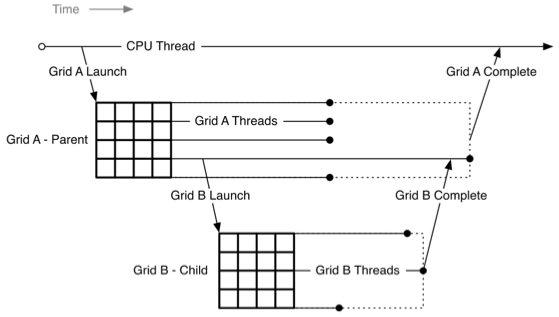
\includegraphics[width=0.65\linewidth]{figure/session-5/nesting-of-grids.png}
    \end{figure}
    
\end{frame}


\begin{frame}{Example -- Recall reduction and the main bottleneck}

\begin{columns}[t]
    \begin{column}{.5\textwidth}
        \begin{figure}
            \centering
            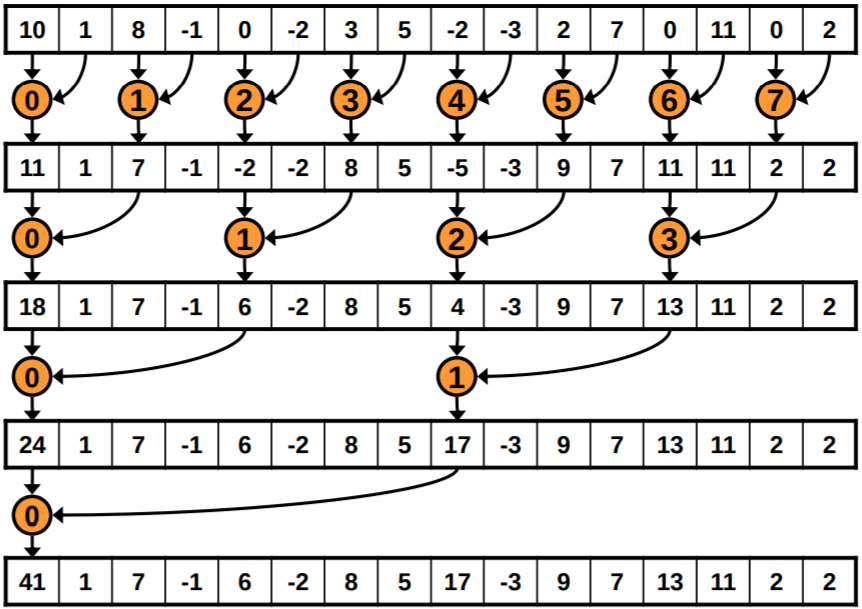
\includegraphics[width=0.9\columnwidth]{figure/session-2/reduction.png}
        \end{figure}
    \end{column}
    \begin{column}{.52\textwidth}
    {\small
    \begin{itemize}\setlength\itemsep{1em}
        \item Had to synchronize threads on each reduction step
        \item Could only synchronize within a block (1024 threads)
        \item Could handle larger data ($N > 2048$) by striding, calling the kernel multiple times, or by using multiple blocks and \inline{atomicMax()}, among others
    \end{itemize}
    }
    \end{column}
\end{columns}

\end{frame}


\begin{frame}{Example -- dynamic parallelism for 2D array reduction}

    \begin{figure}[t]
        \centering
        

\begin{tikzpicture}[]


%%% GRID %%%%%%%%%%%%%%%%%%%%%%%%%%%%%%%%%%%%%%%%%%%%%%%%%%%%%%%%%%%%%%%%%

\def\rowheight{0.5}
\def\rowwidth{0.5}

\def\delta{0.2};

%%% Grid - lines and fill

\draw[] (0,0) rectangle ++(10*\rowwidth,6*\rowheight);

\filldraw[draw=black, fill=black!05!white] (0,5*\rowheight) rectangle ++(10*\rowwidth,\rowheight);
\filldraw[draw=black, fill=black!20!white] (0,4*\rowheight) rectangle ++(10*\rowwidth,\rowheight);
\filldraw[draw=black, fill=black!35!white] (0,2*\rowheight) rectangle ++(10*\rowwidth,2*\rowheight);
\filldraw[draw=black, fill=black!50!white] (0,\rowheight) rectangle ++(10*\rowwidth,\rowheight);
\filldraw[draw=black, fill=black!65!white] (0,0) rectangle ++(10*\rowwidth,\rowheight);

\draw[] (0,0) rectangle ++(1*\rowwidth,6*\rowheight);
\draw[] (1*\rowwidth,0) rectangle ++(1*\rowwidth,6*\rowheight);
\draw[] (8*\rowwidth,0) rectangle ++(1*\rowwidth,6*\rowheight);
\draw[] (9*\rowwidth,0) rectangle ++(1*\rowwidth,6*\rowheight);


%%% Grid - annotations

\node[black, anchor=center, align=center, font=\footnotesize] at (5*\rowwidth,5.5*\rowheight) {Child kernel 0};
\node[black, anchor=center, align=center, font=\footnotesize] at (5*\rowwidth,4.5*\rowheight) {Child kernel 1};

\node[black, anchor=center, align=center, font=\footnotesize] at (5*\rowwidth,1.5*\rowheight) {Child kernel N-2};
\node[black, anchor=center, align=center, font=\footnotesize] at (5*\rowwidth,0.5*\rowheight) {Child kernel N-1};


%%% Thread annotations

\foreach \i in {0, 4} {

    % Parent
    \draw[black] 
    (0,\i*\rowheight+0.5*\rowheight) --++
    (-\delta,0) --++
    (0,\rowheight) --++
    (\delta, 0);
    \draw[black] (-\delta, \i*\rowheight+1*\rowheight) --++(-\delta, 0);

    % Child
    \draw[black] 
    (\i*2*\rowheight+0.5*\rowheight, 6*\rowheight) --++
    (0, \delta) --++
    (\rowheight, 0) --++
    (0, -\delta);
    \draw[black] (\i*2*\rowheight+1*\rowheight, 6*\rowheight+\delta) --++(0, \delta);

}

\node[black, anchor=east, align=right] at (-2*\delta, 5*\rowheight) {t$_\text{0}$};
\node[black, anchor=east, align=right] at (-2*\delta, 1*\rowheight) {t$_\text{M/2 - 1}$};

\node[black, anchor=south, align=center] at (1*\rowwidth, 6*\rowheight + 1.5*\delta) {t$_\text{m(+1), 0}$};
\node[black, anchor=south, align=center] at (9*\rowwidth, 6*\rowheight + 1.5*\delta) {t$_\text{m(+1), N/2 - 1}$};

\node[black, anchor=center, align=center, font=\footnotesize] at (5*\rowwidth,3*\rowheight) {\dots};


\end{tikzpicture}

    \end{figure}
    
\vspace{1em}
\uncover<2->{Requires at least compute capability 3.5 (lab PCs have 3.0)}

\end{frame}



\section{Asynchronous operation}

\begin{frame}{Offload to GPU (B) without blocking the CPU (A)}

\begin{figure}
    \centering
    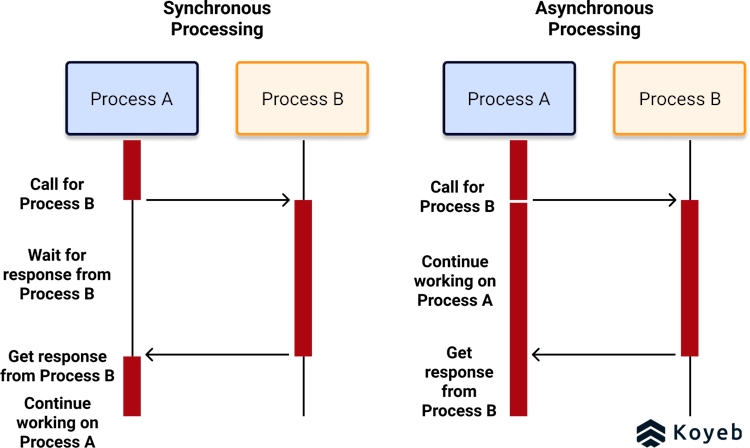
\includegraphics[width=0.7\linewidth]{figure/session-5/sync-vs-async-1.png}
\end{figure}

\vspace{-2em}

{\tiny \href{https://www.koyeb.com/blog/introduction-to-synchronous-and-asynchronous-processing}{Image from Koyeb}}

\end{frame}


\begin{frame}[fragile]{(A)synchronous memory copying}

\begin{lstlisting}[language=C++]
// Copy memory synchronously (wait/block till finished)
cudaMemcpy ( dst, src, count, kind );
...
// Copy memory asynchronously (no waiting, continue with CPU code)
cudaMemcpyAsync ( dst, src, count, kind, stream );
\end{lstlisting}

\vspace{0.5em}

\href{https://docs.nvidia.com/cuda/cuda-runtime-api/group__CUDART__MEMORY.html}{A handy link to the CUDA API reference}

\end{frame}


\begin{frame}[fragile]{Kernel invocation is asynchronous}

\begin{lstlisting}[language=C++]
// This is an asynchronous call by default
foo<<<blk, thr>>>(...);
...
// Can synchronize manually (wait till GPU finished all of its tasks) 
cudaDeviceSynchronize();

\end{lstlisting}

\end{frame}


\begin{frame}[fragile]{Kernel invocation is asynchronous}

\begin{lstlisting}[language=C++]
cudaEvent_t start, stop;
cudaEventCreate(&start);
cudaEventCreate(&stop);

cudaEventRecord(start);

foo<<<blk, thr>>>(...);

cudaEventRecord(stop);

// This also waits 
cudaEventSynchronize ( stop );
\end{lstlisting}

\vspace{0.5em}

Think of a stack (bottom up): \inline{start}, \inline{foo}, \inline{stop}

\end{frame}


\begin{frame}[fragile]{The "GPU call stack" is ordered}

Copy memory to GPU, execute, and copy back to CPU in this order and without blocking the CPU
\vspace{0.5em}

\begin{lstlisting}[language=C++]
// To GPU
cudaMemcpyAsync ( dst, src, count, kind, stream );

// Execute
foo<<<blk, thr>>>(...);

// Back to CPU
cudaMemcpyAsync ( dst, src, count, kind, stream );

\end{lstlisting}

\end{frame}


\begin{frame}[fragile]{CUDA streams}

There can be more than one such "call stack", called a stream to (example):

\vspace{0.5em}
\begin{itemize}\setlength\itemsep{0.5em}
    \item Distinguish between GPU calls (a call for each incoming request/user)
    \item Prioritize certain processing (video rendering vs. video statistics)
\end{itemize}
\vspace{0.25em}

\begin{lstlisting}[language=C++]
// Last argument is the stream
cudaMemcpyAsync ( dst, src, count, kind, stream );

// Last argument, again is the stream
foo<<<blk, thr, shared_size, stream>>>(...);

// Wait for the stream to complete
cudaStreamSynchronize( stream )
\end{lstlisting}

\end{frame}



\section{Exercise}

\begin{frame}{Sync vs async execution comparison}

We will revisit reduction:
\vspace{0.25em}
\begin{itemize}\setlength\itemsep{0.5em}
    \item Perform \inline{sum}, \inline{prod}, \inline{min}, and \inline{max}
    \item Process 4 independent arrays
    \item Use a for loop to generate each of the arrays
    \item Approach 1: do all of this in sequence, synchronously
    \item Approach 2: do array generation while the previous data is being asynchrounously on the GPU
    \item Compare the total execution time (including CPU code)
\end{itemize}

\end{frame}


\begin{frame}{The exercise in figure form}

\begin{figure}
    \centering
    

\begin{tikzpicture}[]


\def\lineHeight{0.5}
\def\xOne{0}
\def\xTwo{8}


%%% GRID %%%%%%%%%%%%%%%%%%%%%%%%%%%%%%%%%%%%%%%%%%%%%%%%%%%%%%%%%%%%%%%%%

\node[anchor=south] at (\xOne, 0) {Sync};
\node[anchor=south] at (\xTwo, 0) {Aync};


%%% Synchronous

\draw[blue, ultra thick] (\xOne, 0) --++(0, -\lineHeight);
\draw[blue, ultra thick, dotted] (\xOne, -\lineHeight) --++(0, -\lineHeight);

\draw[red, ultra thick] (\xOne, -2*\lineHeight) --++(0, -\lineHeight);
\draw[red, ultra thick, dotted] (\xOne, -3*\lineHeight) --++(0, -\lineHeight);

\draw[cyan, ultra thick] (\xOne, -4*\lineHeight) --++(0, -\lineHeight);
\draw[cyan, ultra thick, dotted] (\xOne, -5*\lineHeight) --++(0, -\lineHeight);

\draw[magenta, ultra thick] (\xOne, -6*\lineHeight) --++(0, -\lineHeight);
\draw[magenta, ultra thick, dotted] (\xOne, -7*\lineHeight) --++(0, -\lineHeight);


%%% Asynchronous

\draw[blue, ultra thick] (\xTwo, 0) --++(0, -\lineHeight);
\draw[blue, ultra thick, dotted] (\xTwo+0.2, -\lineHeight) --++(0, -\lineHeight);

\draw[red, ultra thick] (\xTwo, -\lineHeight) --++(0, -\lineHeight);
\draw[red, ultra thick, dotted] (\xTwo+0.2, -2*\lineHeight) --++(0, -\lineHeight);

\draw[cyan, ultra thick] (\xTwo, -2*\lineHeight) --++(0, -\lineHeight);
\draw[cyan, ultra thick, dotted] (\xTwo+0.2, -3*\lineHeight) --++(0, -\lineHeight);

\draw[magenta, ultra thick] (\xTwo, -3*\lineHeight) --++(0, -\lineHeight);
\draw[magenta, ultra thick, dotted] (\xTwo, -4*\lineHeight) --++(0, -\lineHeight);


%%% Annotations


\node[blue, anchor=east, align=right, font=\footnotesize] at (\xOne-0.2, -0.5*\lineHeight) {Prepare array for sum};
\node[blue, anchor=east, align=right, font=\footnotesize] at (\xOne-0.2, -1.5*\lineHeight) {Execute sum and get result};

\node[red, anchor=east, align=right, font=\footnotesize] at (\xOne-0.2, -2.5*\lineHeight) {Prepare array for prod};
\node[red, anchor=east, align=right, font=\footnotesize] at (\xOne-0.2, -3.5*\lineHeight) {Execute prod and get result};

\node[cyan, anchor=east, align=right, font=\footnotesize] at (\xOne-0.2, -4.5*\lineHeight) {Prepare array for min};
\node[cyan, anchor=east, align=right, font=\footnotesize] at (\xOne-0.2, -5.5*\lineHeight) {Execute min and get result};

\node[magenta, anchor=east, align=right, font=\footnotesize] at (\xOne-0.2, -6.5*\lineHeight) {Prepare array for max};
\node[magenta, anchor=east, align=right, font=\footnotesize] at (\xOne-0.2, -7.5*\lineHeight) {Execute max and get result};



\draw[-{angle 60}] 
(\xOne+0.5, -3*\lineHeight) -- 
(\xTwo-0.5, -3*\lineHeight)
node[midway, above] {CPU and GPU run in parallel}
node[midway, below] {Less blocking (waiting)};



\end{tikzpicture}

\end{figure}

\end{frame}


\begin{frame}[fragile]{Pointers}

\begin{itemize}\setlength\itemsep{0.75em}
    \item You already have the reduction kernel from exercise 2
    \item Implement summation, multiplication, and minimum detection
    \item Can use the same kernel and change only the computation part see below (or point to a different \inline{__device__} function each time)
\end{itemize}
\vspace{0.5em}

\begin{lstlisting}[language=C++]
__global__ foo(...){
    ...
    #if KERNEL==0
    #   val = ... + ...
    #else
    #   val = ... * ...
    #endif
}
\end{lstlisting}

\end{frame}


\begin{frame}[fragile]{Pointers continued}

\begin{itemize}\setlength\itemsep{0.75em}
    \item Implement a workflow where you define and populate an array on the CPU, before migrating it to the GPU and executing the kernel function.
    \item Do this 4 times, once for each operation: sum, prod, min, and max.
    \item Perhaps make 2 CPU functions - one which calls the kernel(s) synchronously, one after the other, and one that calls them while preparing the data for the next kernel.
    \item Call the two functions from \inline{main()} and get the execution time using the Chrono library (see cheatsheet).
    \item Make sure to synchronize before stopping the timer.
\end{itemize}

\end{frame}



\end{document}
